\documentclass[DIV=12]{scrartcl}

\usepackage[english]{babel}
\usepackage[utf8]{inputenc}
\usepackage[T1]{fontenc}
\usepackage{lmodern}
\usepackage{csquotes}
\usepackage{graphicx}
\usepackage{tabularx}
\usepackage{booktabs}
\usepackage{color}
\usepackage{listings}
\usepackage{hyperref}
\usepackage{microtype}

%%%%%%% OWN PACKAGES %%%%%%%
\usepackage{biblatex}
\addbibresource{references.bib}
\usepackage{subfig}
%%%%%%% END OWN PACKAGES %%%%%%%


% Define user colors using the RGB model
\definecolor{dunkelgrau}{rgb}{0.8,0.8,0.8}
\definecolor{grau}{rgb}{0.9,0.9,0.9}
\definecolor{hellgrau}{rgb}{0.95,0.95,0.95}

\newcommand{\tbx}{tb17}
\newcommand*{\tip}{\emph}
\newcommand*{\tool}{\texttt}

%%%% environment bash %%%%%%%%%%%%%%%%%%%%%%%%%%%%%%%%%%%%%%%%%%%%%%%%%%%
\lstset{ %
    language=bash,
    backgroundcolor=\color{grau},
    captionpos=t,
    escapeinside={\#*}{*)},
%    frame=single,
%    frame=L,
    frame=none,
    keepspaces=true,
%    belowcaptionskip=0em,
%    belowskip=-5pt,
%    aboveskip=1em,
    commentstyle=\normalfont
}
\lstnewenvironment{bash}{}{}  % bash environment
\newcommand{\ibash}{\texttt}  % inline bash
%%%%%%%%%%%%%%%%%%%%%%%%%%%%%%%%%%%%%%%%%%%%%%%%%%%%%%%%%%%%%%%%%%%%%%%%

%%%% environment python %%%%%%%%%%%%%%%%%%%%%%%%%%%%%%%%%%%%%%%%%%%%%%%%
\definecolor{codegreen}{rgb}{0,0.6,0}
\definecolor{codegray}{rgb}{0.5,0.5,0.5}
\definecolor{codepurple}{rgb}{0.58,0,0.82}
\definecolor{backcolour}{rgb}{0.95,0.95,0.92}
\lstdefinestyle{Python}{
    backgroundcolor=\color{backcolour},   
    commentstyle=\color{codegreen},
    keywordstyle=\color{magenta},
    stringstyle=\color{codepurple},
    basicstyle=\scriptsize,
    numberstyle=\tiny\color{black},
    breakatwhitespace=false,         
    breaklines=true,                 
    captionpos=b,                    
    keepspaces=true,                 
    numbers=left,                    
    numbersep=10pt,                  
    showspaces=false,                
    showstringspaces=false,
    showtabs=false,                  
    tabsize=3,
    frame=shadowbox,
    belowskip=10pt,
    aboveskip=10pt
}

%%%%%%%%%%%%%%%%%%%%%%%%%%%%%%%%%%%%%%%%%%%%%%%%%%%%%%%%%%%%%%%%%%%%%%%%

\begin{document}



% Generic describtion of the topic (as short as possible)
\title{Traffic Monitoring in Software Defined Networks}

% All group names
\author{Felix John $<$ujerb@student.kit.edu$>$\\ Mo Shen $<$uzwvg@student.kit.edu$>$ \\ Hermann Krumrey $<$uodxh@student.kit.edu$>$}

% Title of the original paper
\date{Paper: PayLess: A Low Cost Network Monitoring \\ Framework for Software Defined Networks}

\maketitle

\section{Introduction}
% Replace with your paper
This section introduces the reader to the work titled \emph{PayLess: A Low Cost Network Monitoring Framework for Software Defined Networks} by S. Chowdhury, F. Bari, R. Ahmed and R. Boutaba,which was published at the IEEE Network Operations and Management Symposium (NOMS) in 2014.  

% Continue
The paper addresses a common network monitoring problem: the trade-off between monitoring accuracy and network overhead. Increasing the frequency of polling the switches in the network and thereby increasing the monitoring accuracy comes at the cost of greater network overhead. To tackle this problem, the paper proposes a monitoring framework for Software Defined Networks (SDNs), called PayLess. The paper puts forward the following two main contributions: a RESTful API and an adaptive statistics collection algorithm. The API provides a high-level abstract view of the network, allowing to request monitoring statistics through a uniform channel. PayLess itself is comprised of a collection of pluggable components and can easily be extended or modified with custom ones, owing to the well-defined interfaces. Furthermore, the paper features an adaptive statistics collection scheduling algorithm that provides real-time network statistics information while inducing minimal overhead to the network. Finally, the performance of the framework is examined in detail in different simulations in \textit{Mininet}.

\subsection{Implementation}
This section provides details of the implementation as described in the paper. PayLess resides on top of the OpenFlow controller's northbound API, featuring a high-level RESTful API. Network monitoring applications can request the required statistics through the API by registering a \textit{MonitoringRequest} in the form of a JSON object. More specifically, the user can detail the required statistics by specifying the metric or level of aggregation. 

The center piece of the paper is the adaptive statistics collection algorithm that aims at solving the trade-off between monitoring accuracy and network overhead. The pseudocode of this algorithm is depicted in figure \ref{fig:algorithm}. In contrast to FlowSense \cite{g3.yu2013flowsense}, which makes use of \textit{PacketIn} and \textit{FlowRemoved} messages only, this algorithm requires the controller to send additional \textit{FlowStatisticsRequest} messages to the switch. For every \textit{PacketIn} message the algorithm adds a new flow to a hash table, including the corresponding switch, port and an initial statistics collection timeout value. This table is used to keep track of the active flows in the network, indexed by the flow's respective timeout value. Additionally, the flows that exhibit the same timeout value are grouped together in the same bucket inside the hash table. The following two scenarios are distinguished: Either the timeout value is surpassed or the flow expires within the specified timeout. If the flow expires, the controller will consequently receive the statistics in a \textit{FlowRemoved} message. 
Otherwise, in response to the timeout of a flow, the controller sends a \textit{FlowStatisticsRequest} message to the corresponding switch, requesting the statistics for the flow. Each bucket in the hash table is assigned a worker thread, which is responsible for periodically requesting the statistics in accordance with the timeout value of the bucket. When receiving the corresponding \textit{FlowStatisticsReply} message, the algorithm calculates the difference between the previous and current byte count as well as the difference in duration. Afterwards, the timeout value of each flow is modified, depending on the magnitude of difference in byte count. This adjustment aims at maintaining a higher polling frequency for flows that currently make a significant contribution to the overall link utilization, while setting a lower polling frequency for flows which contribute less.

Furthermore, the algorithm is optimized by batching \textit{FlowStatisticsRequest} messages of flows which show the same timeout value. The algorithm is implemented using the OpenFlow controller Floodlight.

\begin{figure}[]
  \centering
  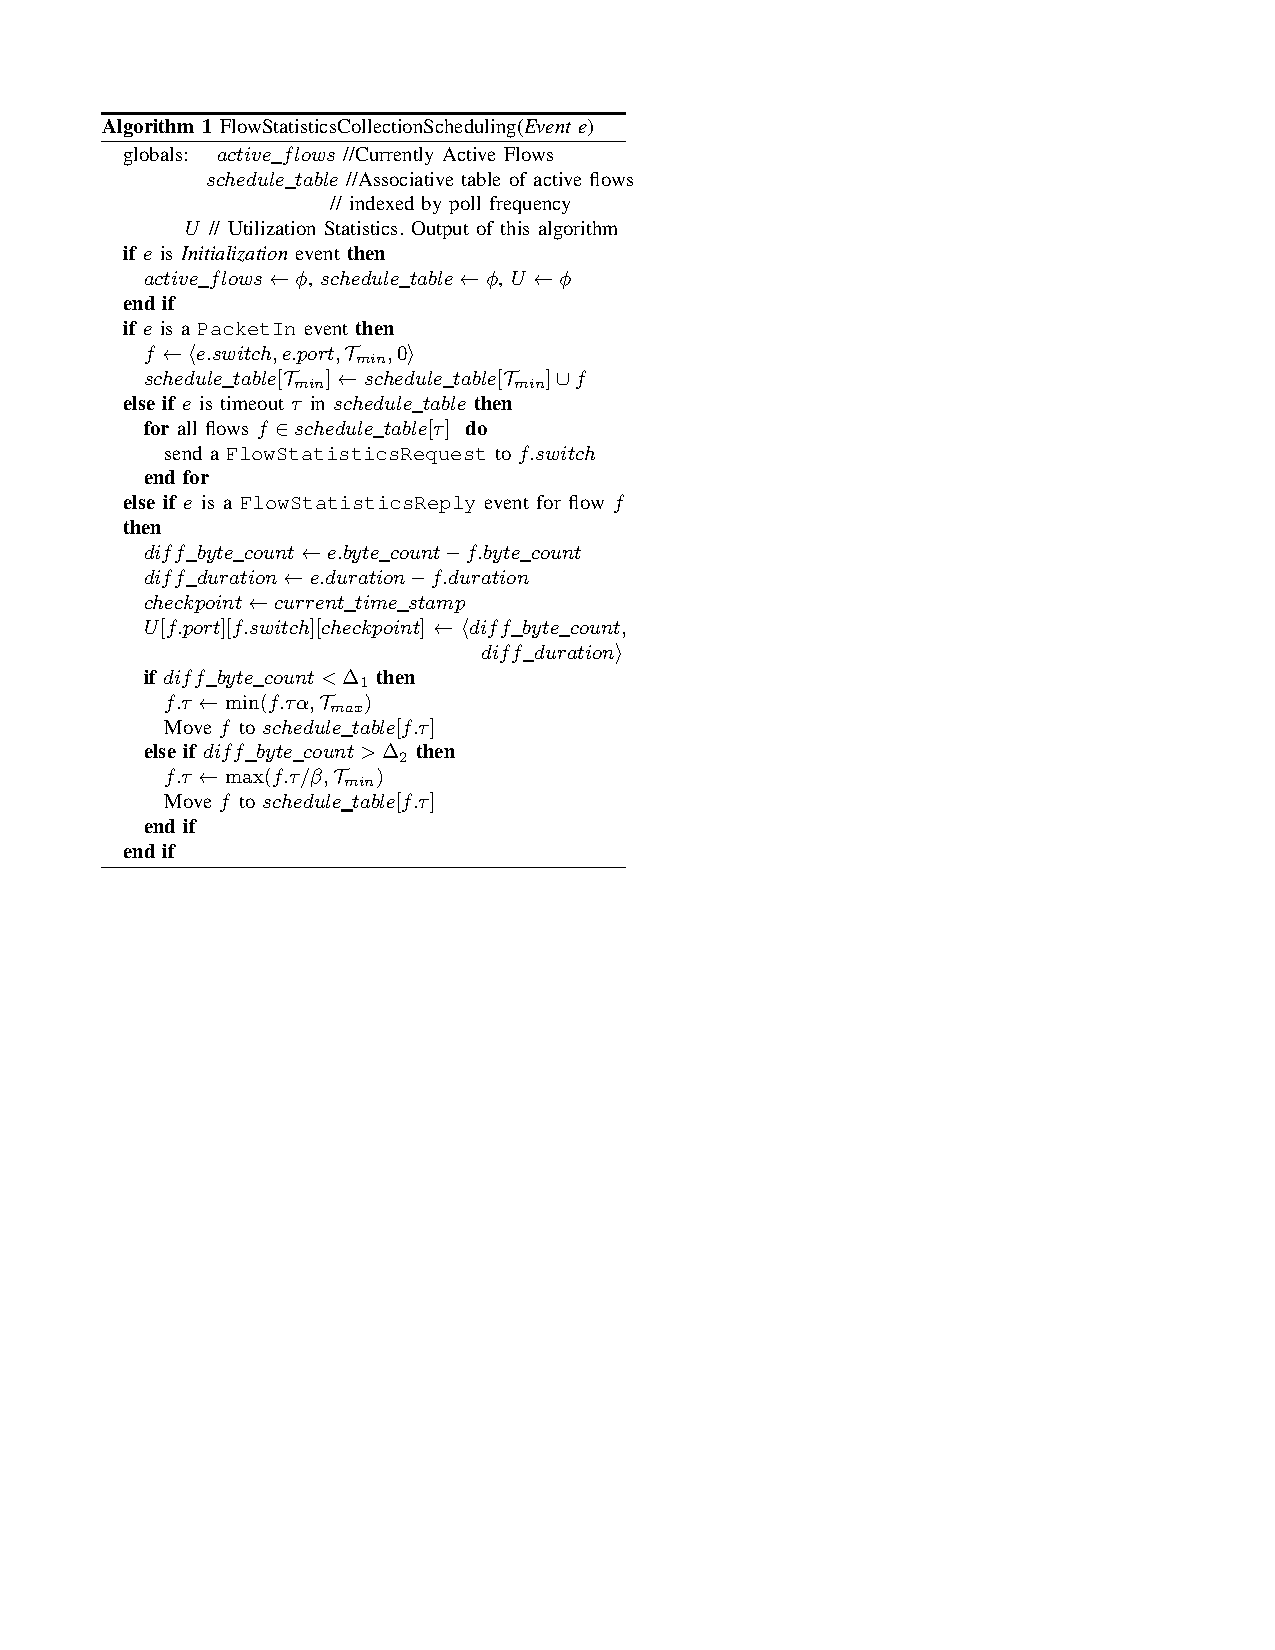
\includegraphics[width=0.5\textwidth]{figures/algorithm_adaptiveAlgorithm.pdf}
  \caption{Pseudocode of the flow statistics scheduling algorithm (from \cite{g3.chowdhury2014payless}) }
  \label{fig:algorithm}
\end{figure}

\subsection{Evaluation Results}
This section described the evaluation results as reported in the paper. The authors conduct a number of different experiments to underscore the effectiveness of the algorithm using \textit{Mininet} to simulate a network and \textit{iperf} for traffic generation. 

\begin{figure}[]
  \centering
  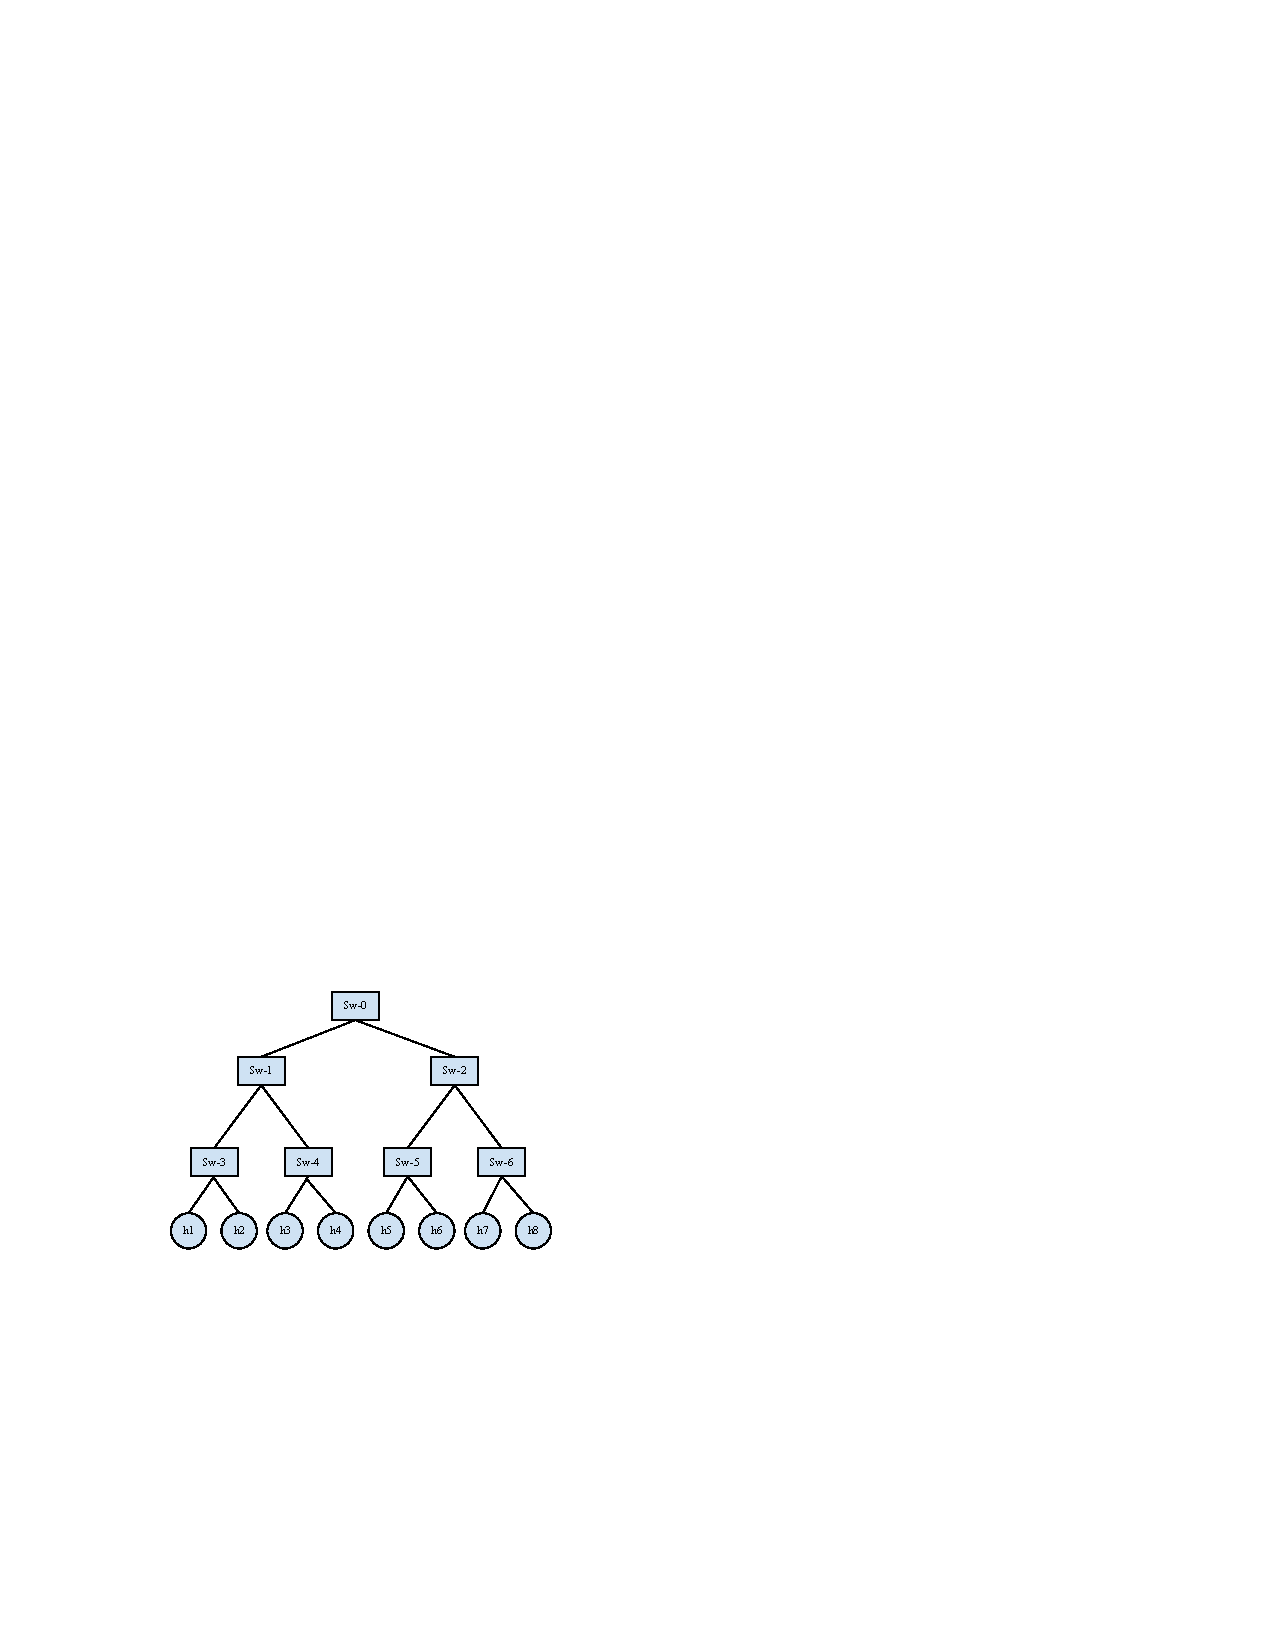
\includegraphics[width=0.6\textwidth]{report/figures/topology_network.pdf}
  \caption{Topology of the network (from \cite{g3.chowdhury2014payless}) }
  \label{fig:topology_network}
\end{figure}

\begin{figure}[t]
  \centering
  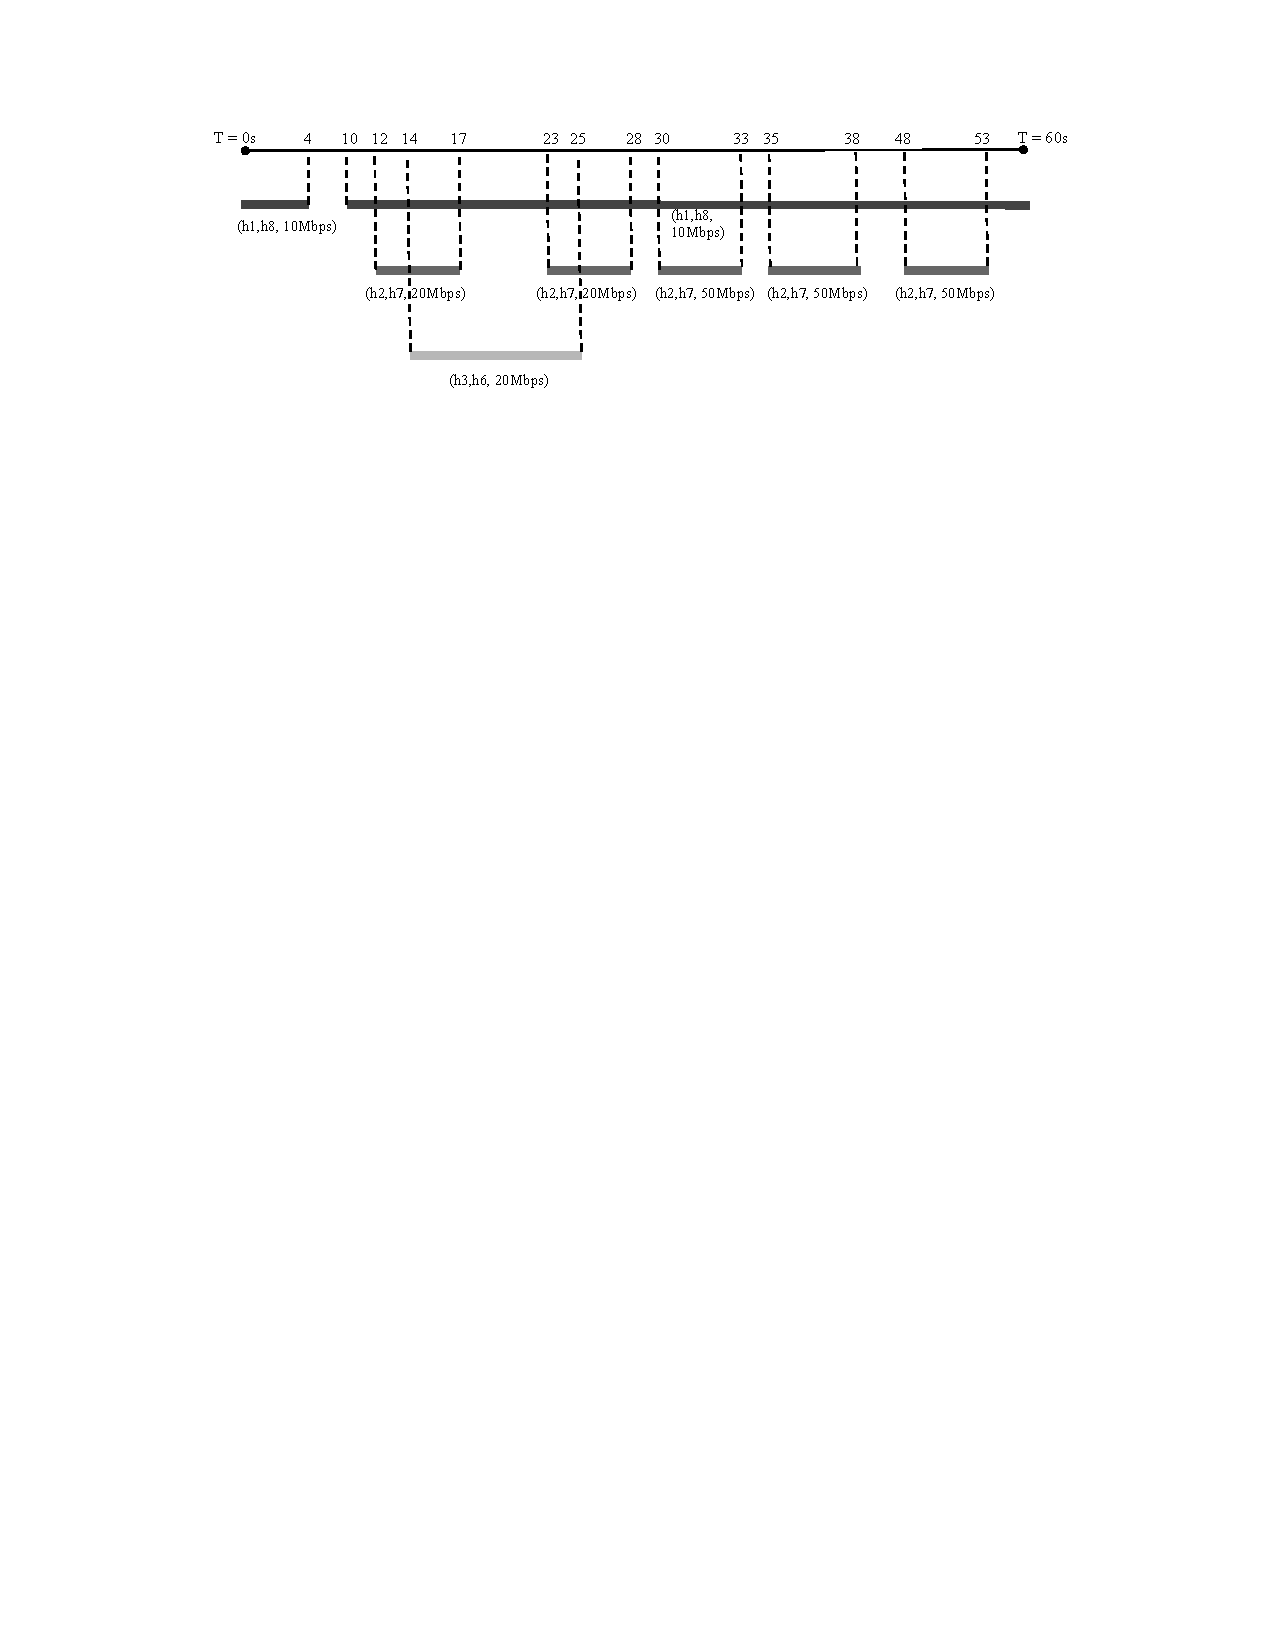
\includegraphics[width=1\textwidth]{report/figures/timing_diagram.pdf}
  \caption{Timing diagram of the generated traffic (from \cite{g3.chowdhury2014payless}) }
  \label{fig:timing_diagram}
\end{figure}

The topology of the network can be seen in figure \ref{fig:topology_network}. The network features 6 switches and 8 different hosts in the 3-level tree topology of the network. The details of the generated traffic are found in figure \ref{fig:topology_network}. UDP traffic flows through the network for a total time of 100 seconds. One experiment focuses on the link utilization between the switches in the network. The performance of the algorithm is compared to a baseline that periodically polls the statistics and the implementation of \cite{g3.yu2013flowsense}. The results are depicted in figure \ref{fig:util_measurement}. 

\begin{figure}[]
  \centering
  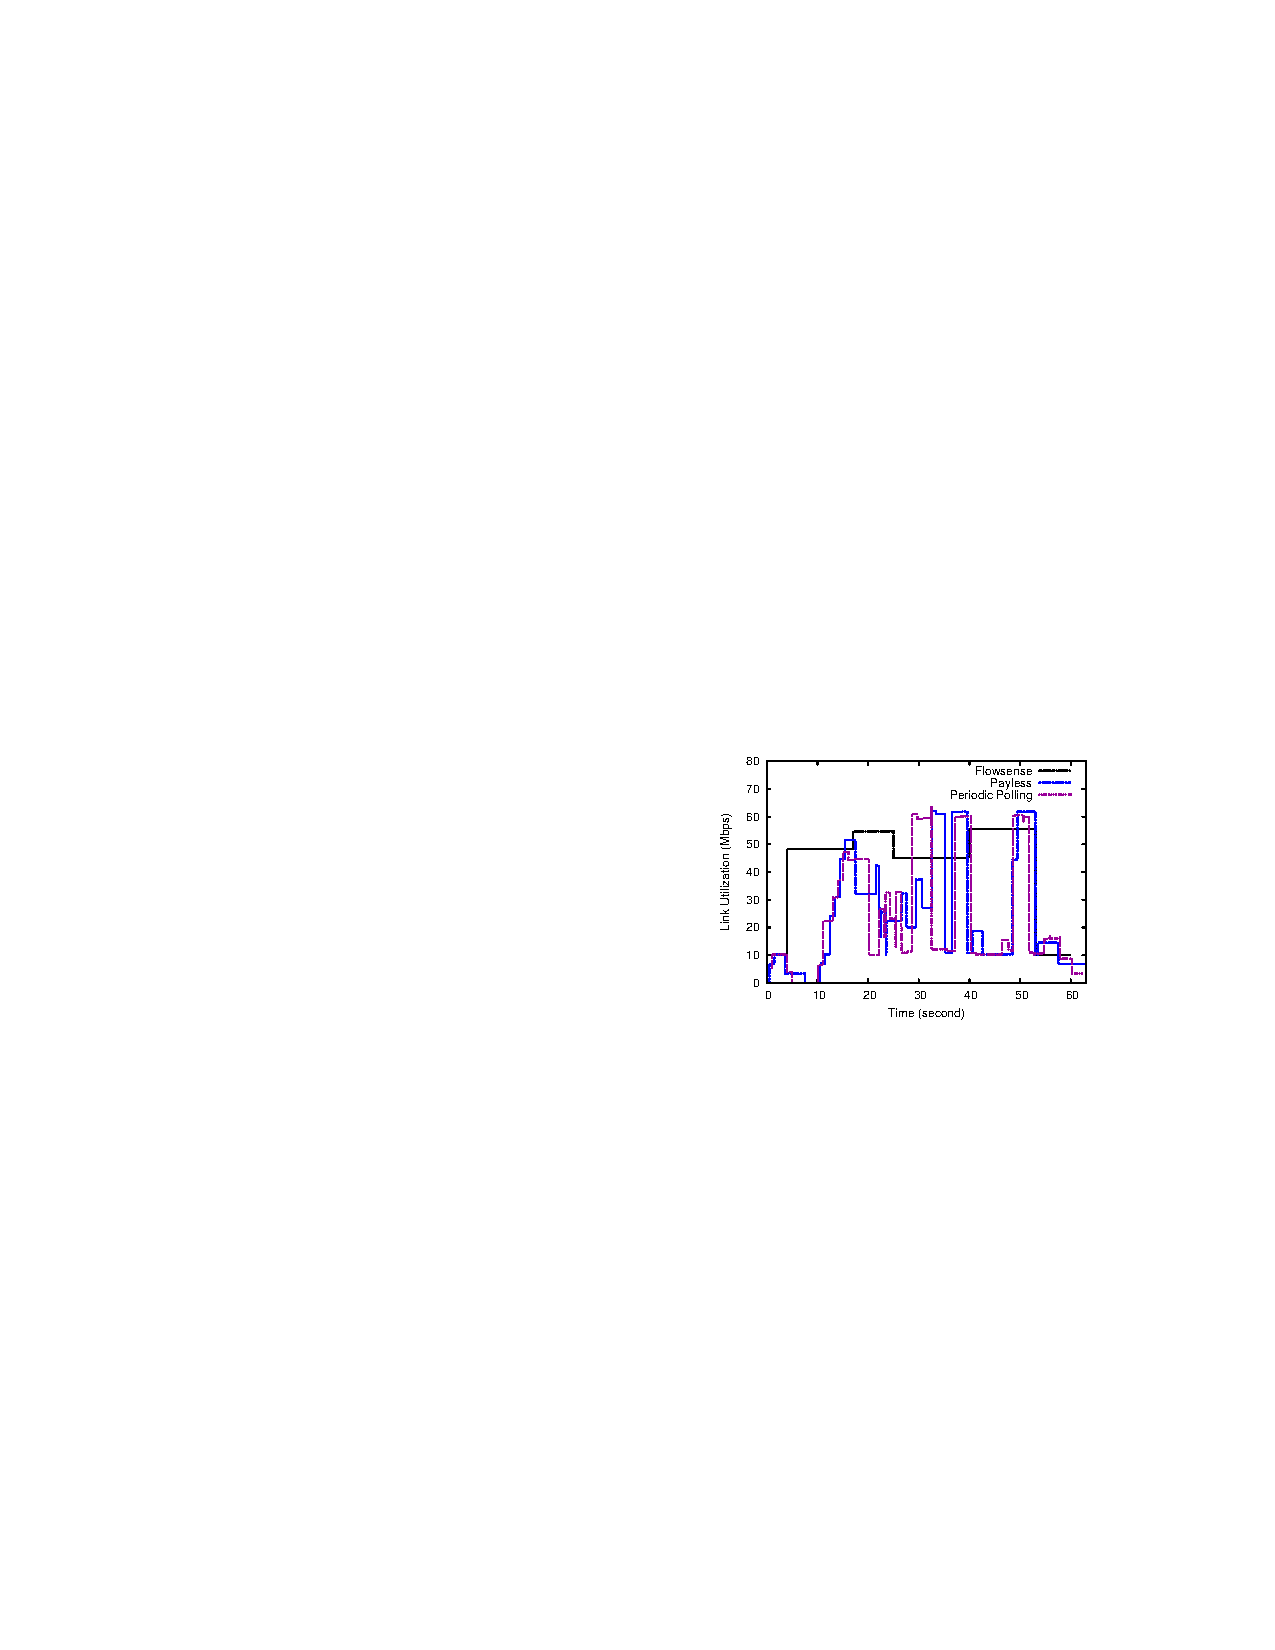
\includegraphics[width=0.6\textwidth]{report/figures/utilization_measurement.pdf}
  \caption{Utilization measurement (from \cite{g3.chowdhury2014payless}) }
  \label{fig:util_measurement}
\end{figure}

\begin{figure}[]
  \centering
  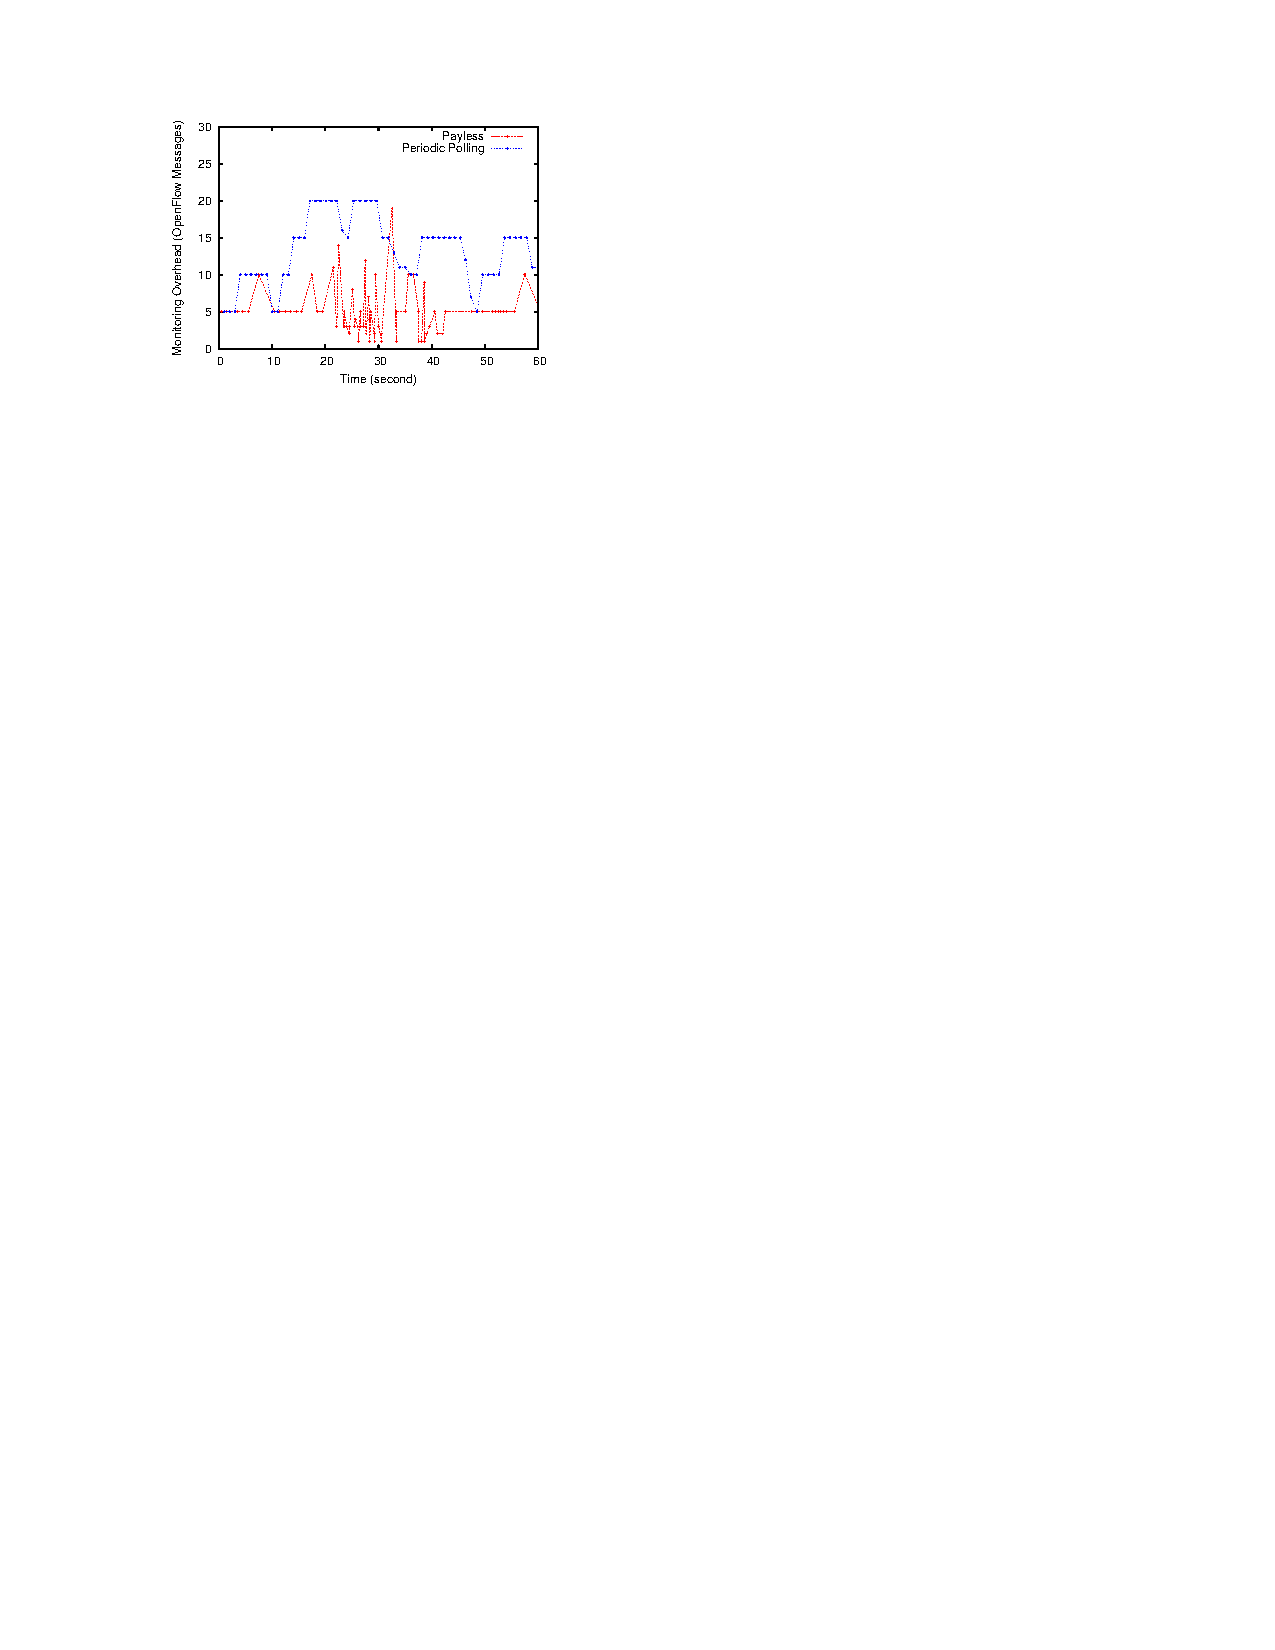
\includegraphics[width=0.6\textwidth]{report/figures/messaging_overhead.pdf}
  \caption{Messaging overhead (from \cite{g3.chowdhury2014payless}) }
  \label{fig:messaging_overhead}
\end{figure}

According to the graphs, the periodic polling most accurately reflects the generated traffic, but inducing a lot of network overhead. Flowsense \cite{g3.yu2013flowsense} on the other hand fails to capture the traffic spikes as it only keeps track of \textit{FlowRemoved} and \textit{PacketIn} messages. In contrast, PayLess closely resembles the measured utilization pattern of the periodic polling. 

Another experiment computes the messaging overhead in terms of the  number of OpenFlow \textit{FlowStatisticsRequest} messages sent during the course of the experiment. The measured overhead of periodic polling and PayLess can be seen in figure \ref{fig:messaging_overhead}. As Flowsense does not make use of \textit{FlowStatisticsRequest} messages, the algorithm is left out in this comparison. PayLess clearly reduces the amount of overhead in the network when compared to the periodic polling. In fact, the proposed algorithm significantly reduces the overhead spikes by adjusting the timeout value and spreading the messages over time. In summary, the evaluation demonstrates the effectiveness of Payless and its capability of maintaining a high monitoring accuracy, while reducing the induced network overhead. 


\section{Report on Reproducibility}

\subsection{Implementation}

This section explores the implementation details of our recreation of the PayLess framework. The major differences and similarities between our implementation and the one
described in the paper are listed in table \ref{tab:differences}. Instead of using the Floodlight controller, we opted to use the Ryu controller due to prior experience with Ryu. The routing algorithm used to determine the flow rules to be installed during experiments was not specified in the paper. For this purpose, we implemented Dijkstra's shortest path algorithm, enabling our implementation to calculate paths for any topology. Our implementation of the monitoring framework generates the statistics output data in JSON format and saves the data to a local file, whereas the implementation in the paper aims to offer access to the monitoring data via the RESTful API.
Our project also includes a rudimentary RESTful API that is based on the RESTful API described in the paper. 
To visualize the raw data, we made use of the \textit{Matplotlib} plotting library. While the original paper relied on \textit{iPerf} to generate experiment traffic, we chose to write our own Python script to set up the traffic for greater flexibility.

\begin{table}[]
    \centering
    \begin{tabular}{|c|c|c|}
        \hline
         Component & Paper & Our Implementation \\
         \hline
         Controller & Floodlight Controller & Ryu Controller \\
         Routing Algorithm & Not specified & Dijkstra's shortest path algorithm \\
         RESTful API & Yes & Yes \\
         Output Format & JSON on demand (via API) & JSON \\
         Visualization & Not specified & matplotlib \\
         Traffic generation & iPerf & Python script \\
         \hline
    \end{tabular}
    \caption{Differences between our implementation and the one in the paper}
    \label{tab:differences}
\end{table}

\subsubsection{Framework}

We developed a framework that supports monitoring of arbitrary network topologies using interchangeable monitoring algorithms.
The framework is implemented in the form of a Python library.
Figure \ref{fig:uml} illustrates the various classes and their relationships with each other as well as important attributes and methods by means of an UML class diagram.

\begin{figure}[]
  \centering
  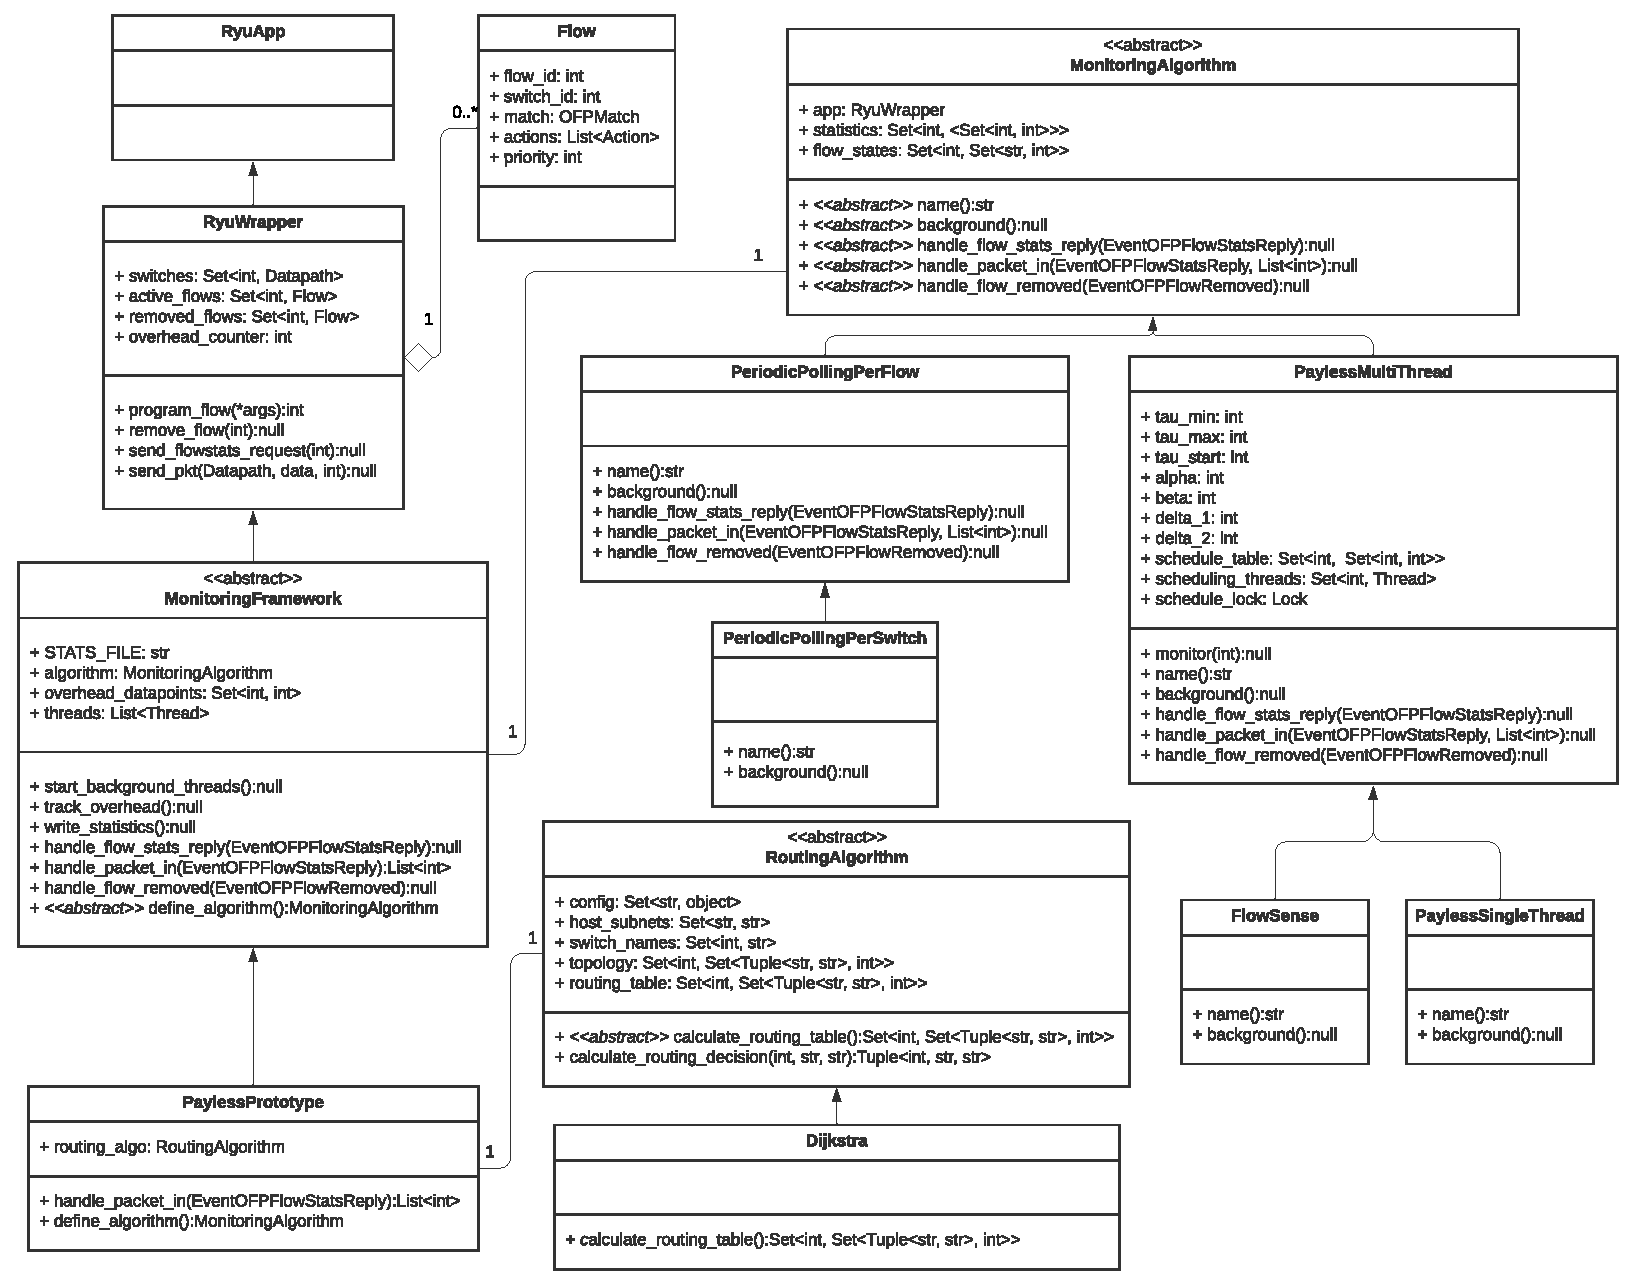
\includegraphics[width=1\textwidth]{report/figures/uml.pdf}
  \caption{UML class diagram of the framework.}
  \label{fig:uml}
\end{figure}

The framework features classes that
inherit from the RyuApp class and add methods as well as fields to simplify the
integration of a monitoring algorithm. This is done in the \textit{RyuWrapper} and
\textit{MonitoringFramework} classes.

Inheriting directly from the \textit{RyuApp} class, the \textit{RyuWrapper} class implements some convenience methods to simplify the tasks of installing new flow rules, forwarding packets and sending flow statistics requests to a switch.
The class also keeps track of connected switches and installed flow rules. All flows are assigned a unique ID. The flow's information is stored
in a so-called Flow object, facilitating the access of information about the flow.
Additionally, the \textit{RyuWrapper} class keeps track of the total number of flow statistics requests sent by the controller.

The \textit{MonitoringFramework} class inherits from the \textit{RyuWrapper} class and integrates an interchangeable monitoring algorithm. The class forwards
\textit{PacketIn}, \textit{FlowStatisticsReply} and \textit{FlowRemoved} messages to the monitoring algorithm. A new thread is also started for any background tasks for the monitoring algorithm. This class also keeps track of the amount of flow statistics requests that were sent each second, which is important for statistics on monitoring overhead over time. Additionally, the class periodically writes the collected monitoring and overhead statistics to a JSON file.

The monitoring algorithms were made interchangeable by encapsulating the algorithm logic in a class that inherits from the abstract class \textit{MonitoringAlgorithm}. Any child class of \textit{MonitoringAlgorithm}
must specify functions that handle the incoming Openflow messages.
Additionally, the \textit{MonitoringAlgorithm} class has to define a method to handles any background logic, running independent of incoming OpenFlow messages.

The library includes an implementation for a periodic polling monitoring algorithm, implemented in the \textit{PeriodicPollingPerFlow} class. Being based on the description in the original paper, this periodic polling algorithm serves as a baseline to which the other monitoring algorithms are compared to. As the name implies, the algorithm periodically polls the switches of any active flows once every second. Beyond that, we provide an extension to periodic polling, namely the \textit{PeriodicPollingPerSwitch} class, which polls each switch every second.

We replicated the adaptive monitoring algorithm presented in the original paper in two different ways. Although both variants implement the algorithm described in the paper, they differ in their approach to threads.
The first variant, namely \textit{PaylessMultiThread}, spawns a new thread for each bucket, while \textit{PaylessSingleThread} makes use of a one single, main background thread. Both variants support modifying the Payless algorithm parameters using constructor parameters. Additionally, we included a simple implementation of FlowSense \cite{g3.yu2013flowsense} in the \textit{FlowSense} class. This algorithm only reacts to incoming \textit{FlowRemoved} messages and does not actively send out flow statistics requests. 

The \textit{PaylessPrototype} class is not part of the library, but rather makes use of the library to create a fully functional SDN application with monitoring functionality.
The class inherits from the \textit{MonitoringAlgorithm} class and can be configured using environment variables to specify the following properties:

\begin{enumerate}
    \item The monitoring algorithm to use
    \item Payless algorithm parameters
    \item Output file path
    \item Topology file path
\end{enumerate}

The \textit{PaylessPrototype} makes use of Dijkstra's shortest path algorithm to calculate appropriate flow rules for incoming packets based on the topology file. Dijkstra's algorithm is encapsulated in the \textit{DijkstraRouting} class, which is a subclass of the \textit{RoutingAlgorithm} class. This construct should support and ease any modification or replacement of the routing algorithm, if required in the future. After the flow rules are calculated, they are installed reactively with an idle timeout of 5 seconds.

\subsubsection{Visualization}

To visualize the resulting monitoring data, we made use of the \textit{Matplotlib} plotting library.
For the sake of visual consistency, we attempted to keep the style and formatting of the generated graphs in line with the style and formatting in the paper.

The visualization of the link utilization statistics ignores any flows that do not match on IPv4 sources and destinations, which in essence means that
the statistics on the default flow rules are not represented.
As the data collected by the monitoring framework are represented as individual events of a specified duration and byte count, the visualization must first prepare the data for display in a continuous graph, as well as normalize the data in regards to the first point of the graph on the time axis.
This is required to effectively compare the graphs of different monitoring algorithms.
Additionally, the unit of time is reduced to seconds, as opposed to milliseconds, which are used in the raw data generated by the monitoring framework.
The link utilization statistics can be bundled in three different ways:

\begin{enumerate}
    \item per flow
    \item per IPv4 match
    \item total link utilization of the network
\end{enumerate}

The visualization of overhead statistics also requires normalized data, however,
the plotting is simpler here, as the statistics are already in a format that
easily translates to a continuous graph.
We included two variants for visualizing overhead statistics.
The cumulative variant shows the total overhead generated by an experiment over time, while the relative variant shows the overhead generated in one particular second. Examples for generated graphs can be found in section \ref{subsec:eval}.

\subsubsection{RESTful API}
Next to the implementation of the statistics collection algorithm, we set up a basic RESTful API similar to what is described in the paper. The API is built using the web framework \textit{Flask} and the database toolkit \textit{SQLAlchemy}. Any client can interact with the API by making use of the API functions by the URIs specified in the paper. More specifically, every network client needs to create a \textit{MonitoringRequest} object and register it with the API. The \textit{MonitoringRequest} contains the details of the desired monitoring statistics and is specified using JSON. The implemented URIs provide the basic CRUD functionality for the \textit{MonitoringRequest} object. In contrast to the paper that can retrieve the data on demand, this API can only fetch the data once it has been generated by the statistics collection algorithm. 
\begin{figure}[]
  \centering
  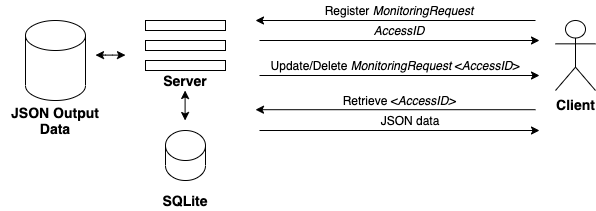
\includegraphics[width=1.0\textwidth]{report/figures/api.png}
  \caption{Architecture of RESTful API}
  \label{fig:api}
\end{figure}
The architecture of the RESTful API can be seen in figure \ref{fig:api}. Each \textit{MonitoringRequest} is separately stored in an \textit{SQLite} database. First, the client has to register his monitoring request, receiving an \textit{AccessID} in return. Afterwards, the client can use this ID to retrieve the desired data or make changes to his initial monitoring request.


\subsection{Environment Setup and Traffic Generation}
Reconstructing the environment setup is as important as the implementation of the framework. Firstly, we want to reproduce and replicate the results presented in the paper. Moreover, we aim to make a more in-depth performance comparison of the various monitoring algorithms by including more scenarios.

We used \textit{Mininet} to set up the network topology and wrote the remote controller based on the \textit{Ryu} framework.
To ease the use of \textit{Mininet} with different network topologies, we wrote a Python script that generates a \textit{Mininet} topology based on a YAML configuration file.

In order to perform the experiments, an appropriate traffic generator is required. A well-designed traffic generator should uniformly transfer data over time and be flexible enough to fit itself into various scenarios.
There are several tools to choose from. First, we considered \textit{trafgen} for traffic generation. It allows to define packets in plain text and the sending behaviour with command line arguments. However, because we faced some difficulties using it outside of \textit{sdn-cockpit}, we abandoned \textit{trafgen} at the very beginning. The second option is the high-level network bandwidth measurement tool, called \textit{iperf}. It is able to generate and analyse the traffic at the same time. This option was also discarded as \textit{iperf} hides the details of how the packets are sent, making the evaluation of the actual utilization of the network difficult. Looking into the implementation of \textit{iperf} could clarify the behaviour, but will also add extra work to the project and it shifts from the topic of SDN too much. As a result, we implemented our own UDP traffic generator to ensure the most fine-grained control.
Under the hood it utilizes raw sockets in the UNIX system.
The script takes a YAML file as input to determine how the traffic should be generated. Additionally, the content of packets can be defined in Python code.
 
\subsection{Evaluation Results}
\label{subsec:eval}

Our goal was to validate the claims made by the original paper as well as finding
any potential scenarios in which the PayLess approach to monitoring can thrive. We also attempted to find any issues with using PayLess for monitoring SDN applications.

\subsubsection{Experiment 1: Recreating Original Experiment}

To confirm the claims made by the original paper, we recreated the
network topology depicted in figure \ref{fig:topology_network} as well as the traffic described in the timing diagram in figure \ref{fig:timing_diagram} that were used in the experiment. Then, we ran the experiment using the periodic polling (PeriodicPollingPerFlow), PayLess (PaylessMultiThread) and FlowSense algorithms and visualized the resulting monitoring data.
The resulting link utilization and network overhead graphs can be seen in figure \ref{fig:experiment1}.

\begin{figure}%
    \centering
    \subfloat[Total Link Utilization]{{
        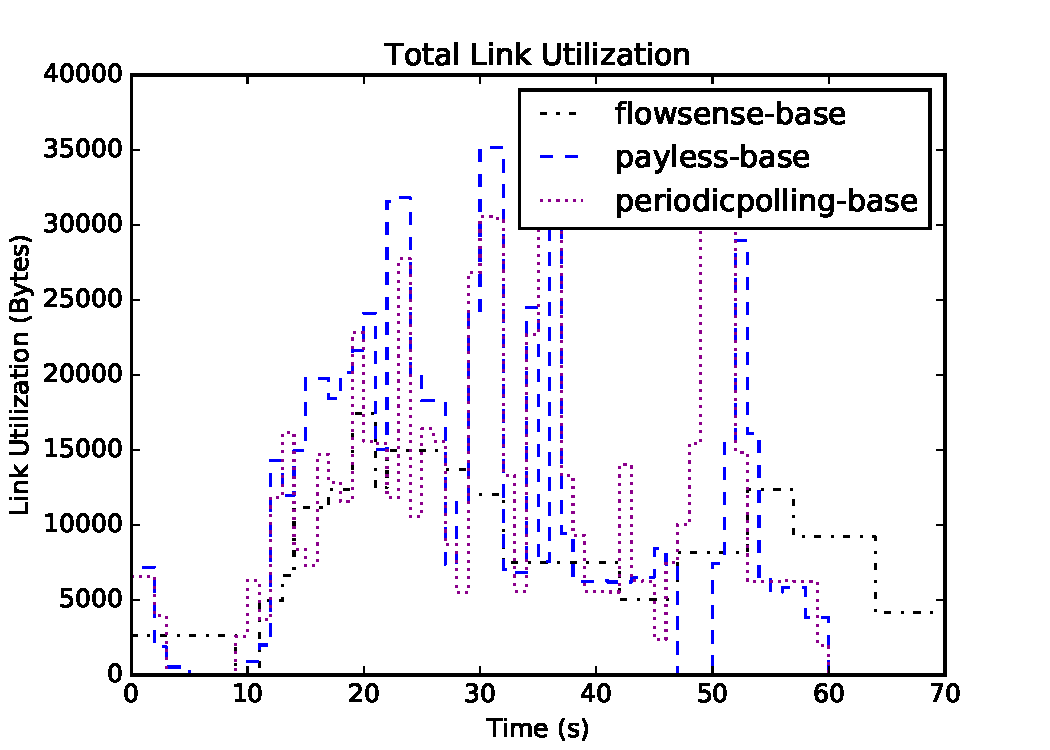
\includegraphics[width=0.5\textwidth]{report/figures/base-link-utilization.pdf}
    }}%
    \subfloat[Relative Network Overhead]{{
        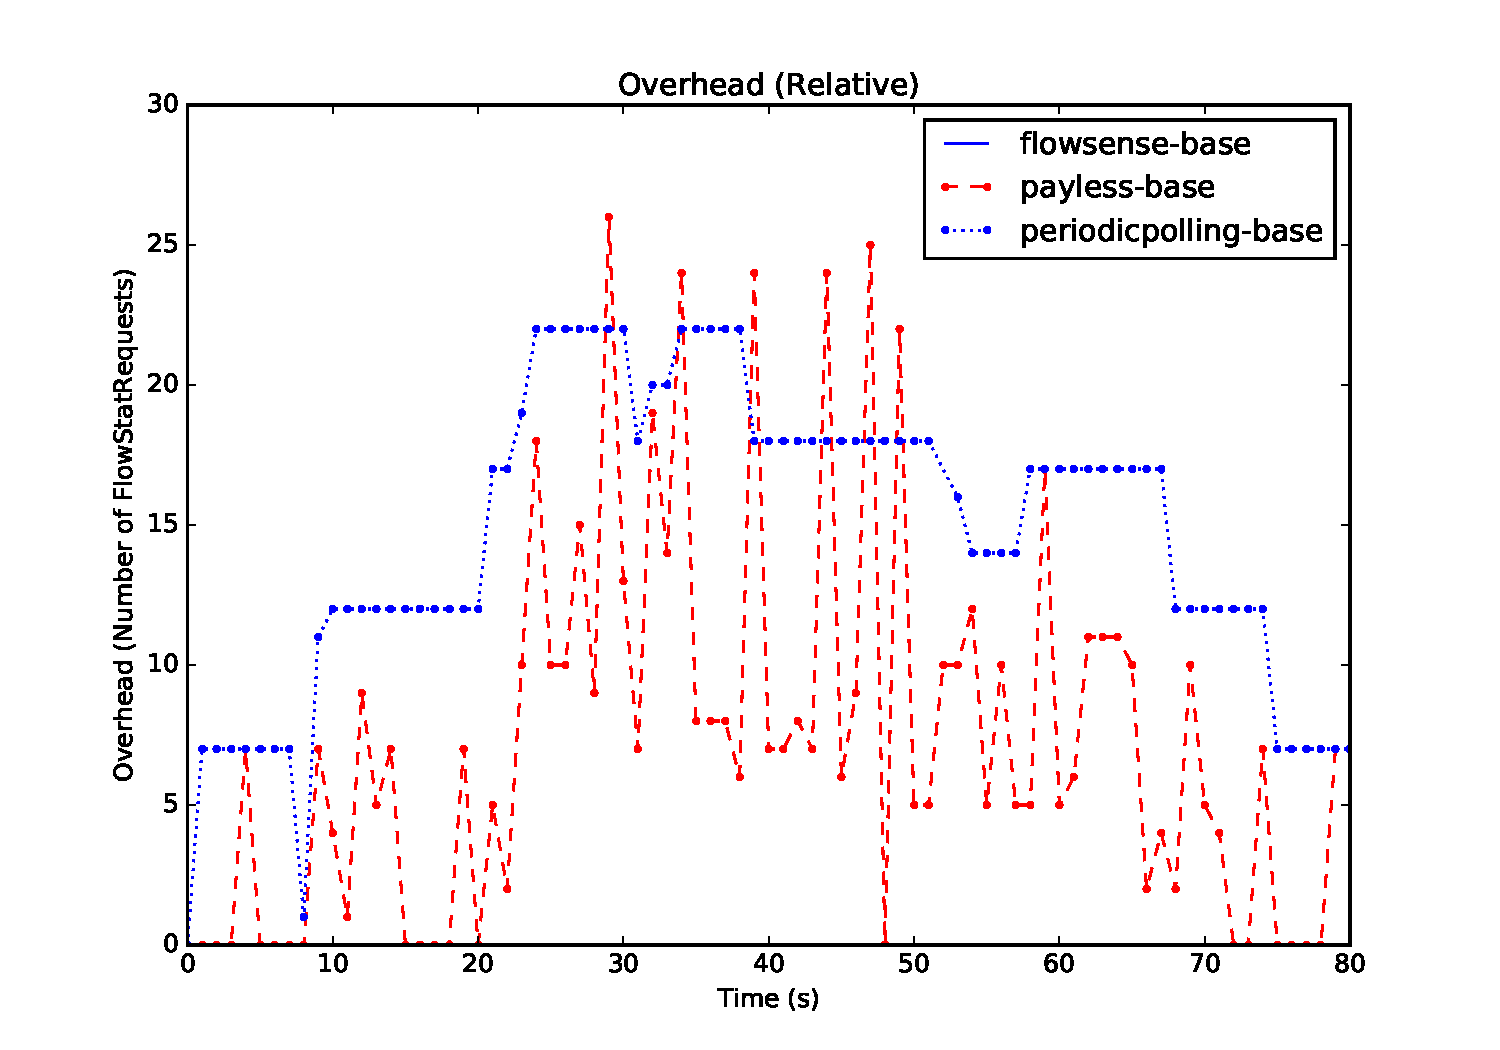
\includegraphics[width=0.5\textwidth]{report/figures/base-relative-overhead.pdf}
    }}%
    \caption{Results for the experiment based on the original paper (experiment 1).}%
    \label{fig:experiment1}%
\end{figure}

The results of this experiment confirm that payless is able to achieve
roughly the same degree of monitoring accuracy for this particular setup as the periodic polling approach while incurring less network overhead at almost every point in time.
Our implementation seems to produce less stable results, with more jitter
than the one depicted in the original paper, which can be observed by comparing 
figures \ref{fig:util_measurement} and \ref{fig:experiment1}a.

\subsubsection{Experiment 2: Experiment with Less Traffic}

We also conducted further experiments. For example, using the very same scenario as before, we reduced the amount of packets sent by the hosts by a factor of around one hundred. The resulting link utilization and monitoring overhead graphs can be seen in figure \ref{fig:experiment2}.

As can be seen in figure \ref{fig:experiment2}b. the PayLess algorithm essentially acts the same way the periodic polling algorithm would if the polling interval were set to 5 seconds. This is due to the fact that the low amount of traffic causes all flows to eventually be assigned to the bucket with the lowest polling frequency. Although the PayLess approach loses some of its accuracy when dealing with less traffic, it produces considerably less network overhead than in the previous scenario. Figure \ref{fig:overhead_compare_base_slow} compares the network overhead generated by PayLess in both of these experiments.

\begin{figure}%
    \centering
    \subfloat[Total Link Utilization]{{
        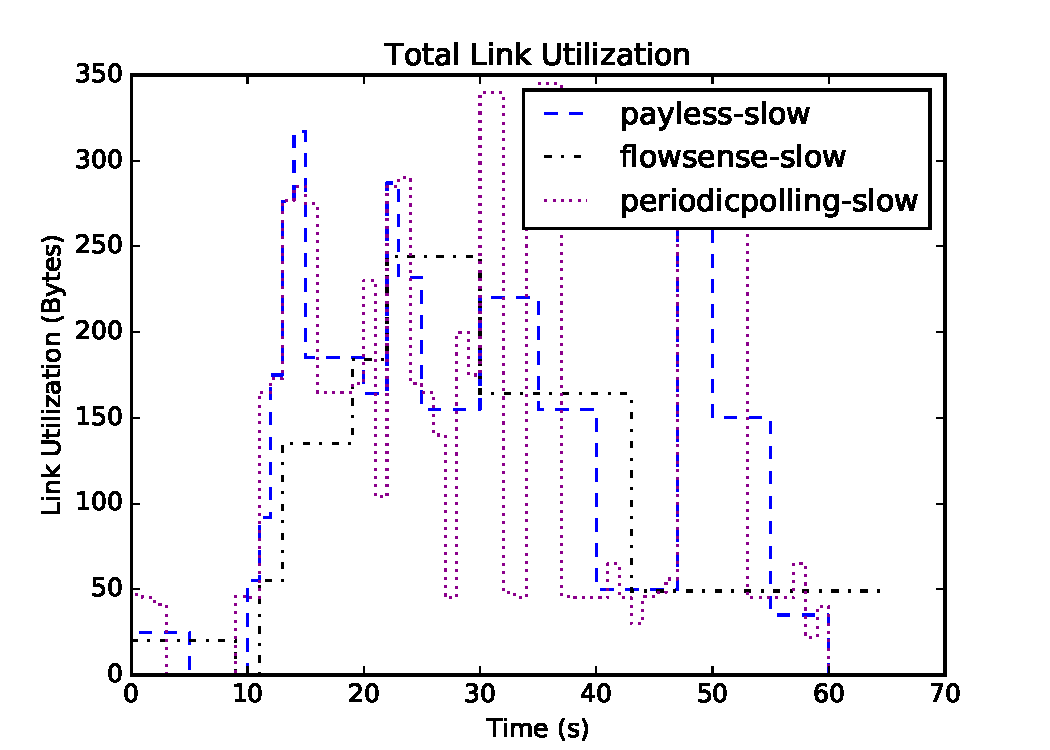
\includegraphics[width=0.5\textwidth]{report/figures/slow-link-utilization.pdf}
    }}%
    \subfloat[Relative Network Overhead]{{
        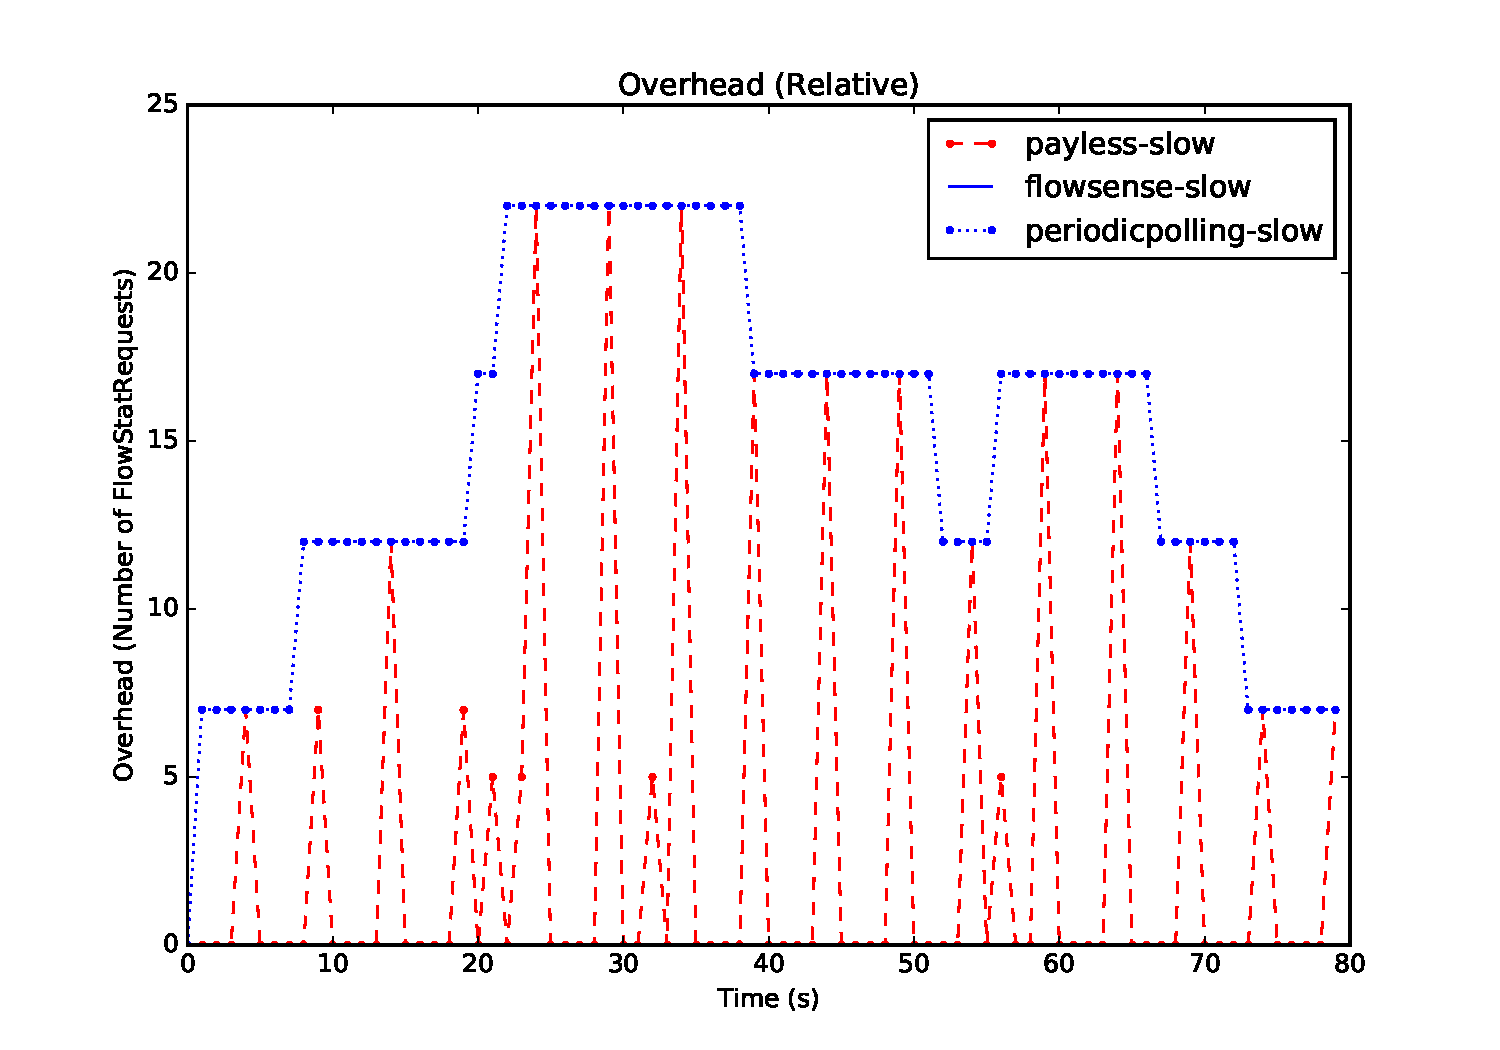
\includegraphics[width=0.5\textwidth]{report/figures/slow-relative-overhead.pdf}
    }}%
    \caption{Results for the experiment using less traffic (experiment 2).}%
    \label{fig:experiment2}%
\end{figure}

\begin{figure}[]
  \centering
  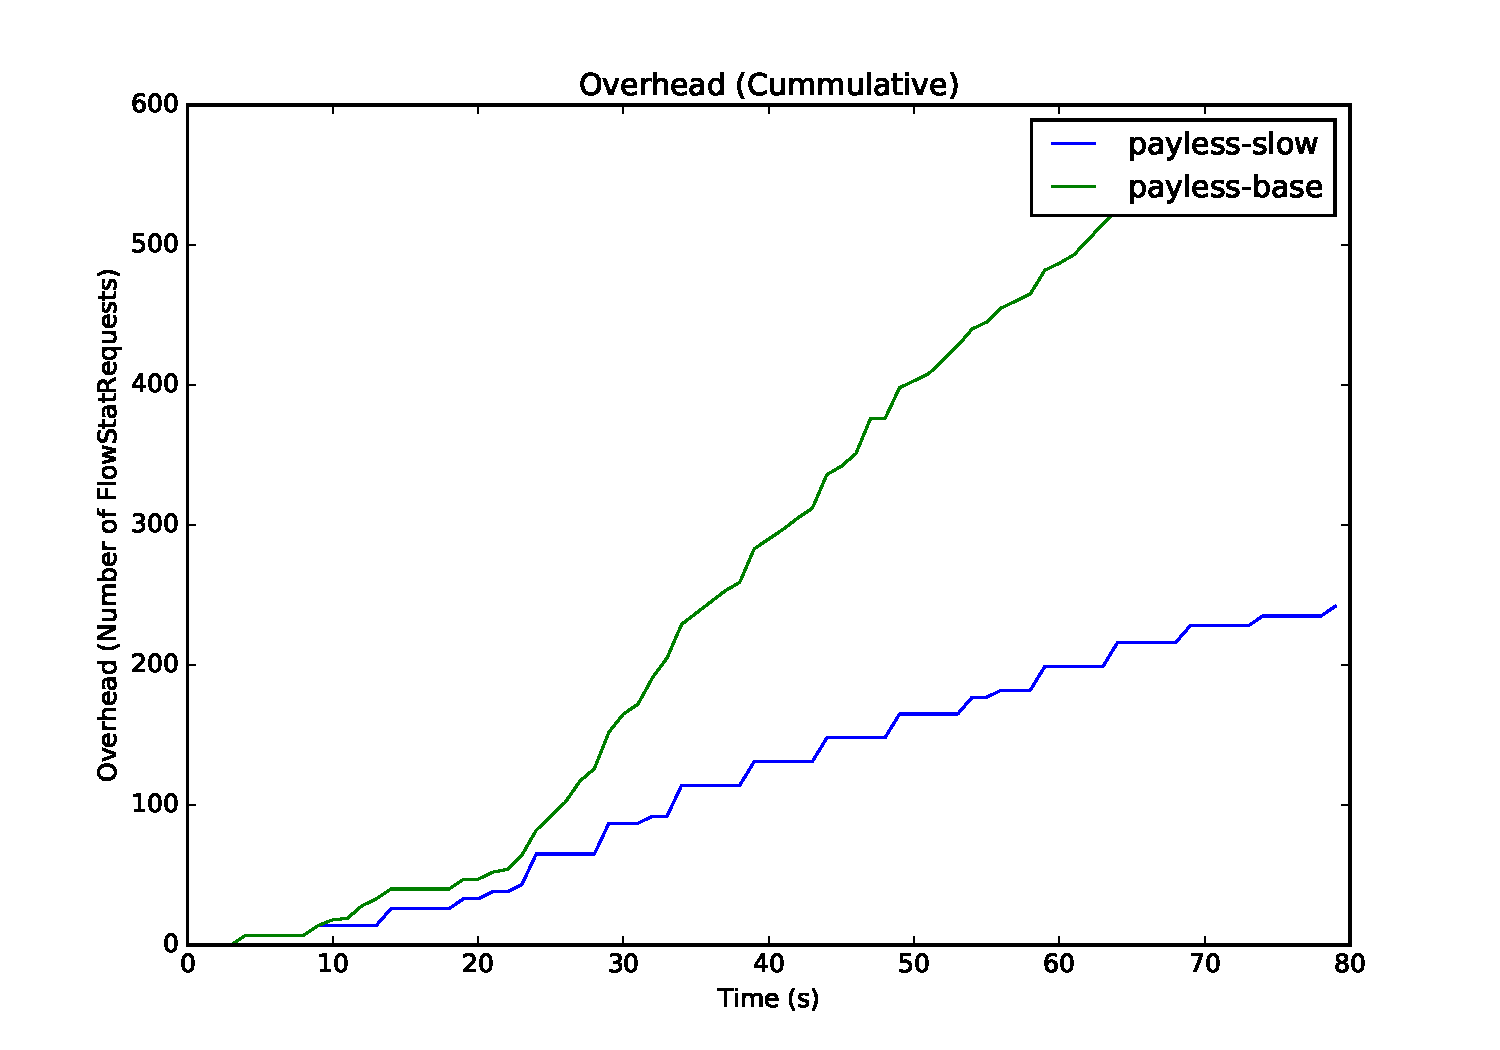
\includegraphics[width=0.5\textwidth]{report/figures/base-slow-overhead-cummulative-compare.pdf}
  \caption{Comparison of cumulative overhead generated by payless during experiment 1 (base-payless) and experiment 2 (slow-payless).}
  \label{fig:overhead_compare_base_slow}
\end{figure}

\subsubsection{Experiment 3: Experiment with Temporary Pause in Traffic}

Another experiment that we conducted is based on a new scenario that includes
two 15 seconds long traffic spikes separated by a 20 second pause in which no new traffic is generated by the sending hosts. This experiment resulted in the link utilization and cumulative overhead graphs seen in figure
\ref{fig:experiment3}.

\begin{figure}%
    \centering
    \subfloat[Total Link Utilization]{{
        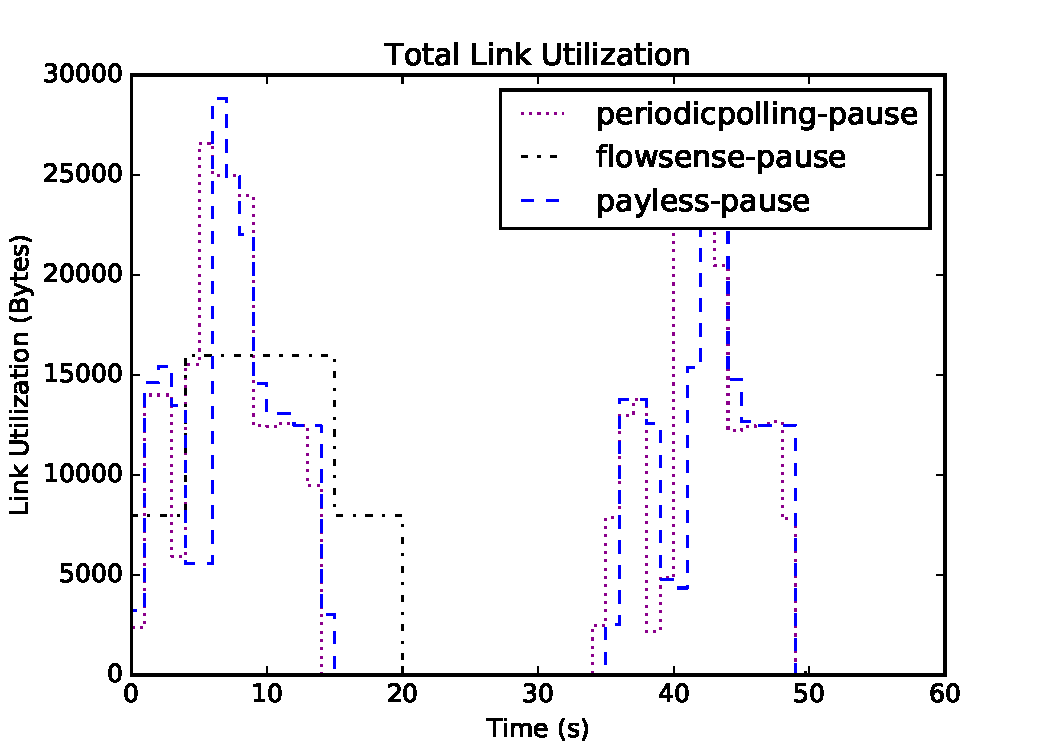
\includegraphics[width=0.5\textwidth]{report/figures/pause-link-utilization.pdf}
    }}%
    \subfloat[Cumulative Network Overhead]{{
        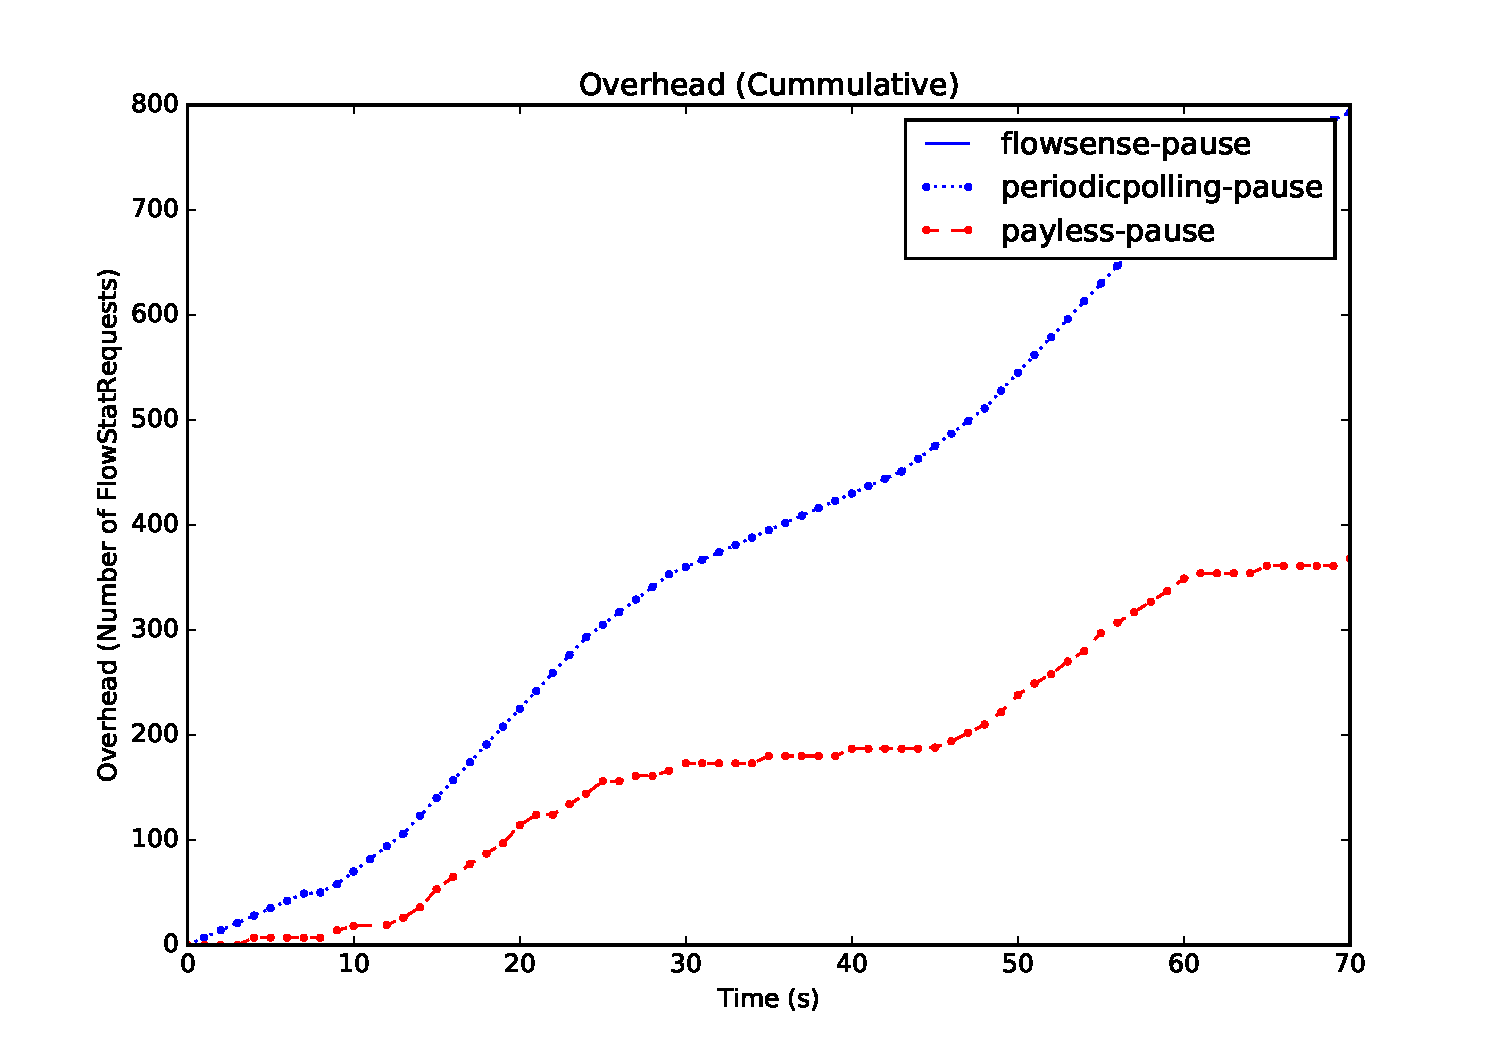
\includegraphics[width=0.5\textwidth]{report/figures/pause-cummulative-overhead.pdf}
    }}%
    \caption{Results for the experiment that includes a 20 second pause in traffic (experiment 3).}%
    \label{fig:experiment3}%
\end{figure}

This experiment demonstrates that PayLess generates noticeably less network overhead than the periodic polling approach during the phase without any new traffic. Additionally, PayLess can compete in terms of monitoring accuracy when compared to the periodic polling approach. 

\subsection{How to Reproduce}

This section describes how to reproduce the evaluation results.
We use vagrant to build and maintain a portable development environment.
A working installation of vagrant is required to successfully proceed with the following steps. Use Git to download all the configuration files and source code.
Then setup the environment as shown in Listing~\ref{lst:setup_vagrant}.

\begin{lstlisting}[float=htbp, caption={Setup vagrant}, label={lst:setup_vagrant}]
git clone https://git.scc.kit.edu/tm-praktika/ppsdn-2020/g3.git
cd g3
vagrant up
vagrant ssh
./setup.sh
\end{lstlisting}

To interact with the framework via RESTful API, start the server with \texttt{python api/app.py} and send requests to \texttt{http://127.0.0.1:3000}.
An example is given in Listing~\ref{lst:request_example}.

\begin{lstlisting}[language=Python, float=htbp, caption={Start Server}, label={lst:request_example}]
import requests
request = {
    "MonitoringRequest": {
        "metric": "utilization",
        "aggregation_level": "switch",
        "monitor": "adaptive"
    }
}
url = 'http://127.0.0.1:3000/'
      'payless/object/monitor_request/register'
res = requests.post(url, json=request)
if res.ok:
    print(res.content)
\end{lstlisting}

Now it is possible to run experiments with the help of the python script \texttt{run\_experiment.py}.
It takes two YAML files, one for the topology and another for traffic generation.
The third argument specifies the algorithm to use for monitoring.
Available options are \texttt{payless}, \texttt{periodicpolling} and \texttt{flowsense}.
The \texttt{-o} option can be used to specify the path to the file in which to store the collected statistics.
Furthermore, one can append \texttt{-d} or \texttt{-v} for debug or verbose output.
To reproduce the experiments conducted in the paper, execute the commands shown in listing \ref{lst:run_experiments}.

\begin{lstlisting}[float=htbp, caption={Run experiments}, label={lst:run_experiments}]
sudo python run_experiment.py \
    scenario/topo-payless.yaml scenario/scene-payless.yaml \
    payless -o payless.json -v
sudo python run_experiment.py \
    scenario/topo-payless.yaml scenario/scene-payless.yaml \
    periodicpolling -o periodicpolling.json -v
sudo python run_experiment.py \
    scenario/topo-payless.yaml scenario/scene-payless.yaml \
    flowsense -o flowsense.json -v
\end{lstlisting}

Visualizing the statistics recorded in JSON format is also convenient with the help of the custom python scripts.
They can be found under the \texttt{bin} folder.
Listing~\ref{lst:visualize_statistics} shows how to generate graphs for the total link utilization and relative overhead and export them to PNG files.

\begin{lstlisting}[float=htbp, caption={Visualize statistics}, label={lst:visualize_statistics}]
g3-link-utilization total \
    payless.json periodicpolling.json flowsense.json \
    -o link_utilization.png
g3-overhead relative \
    payless.json periodicpolling.json flowsense.json \
    -o overhead.png
\end{lstlisting}

We also included \texttt{run\_all.sh}, a script that automatically runs all 
experiments used to generate the graphs in this report.
It saves the monitoring data in a directory named after the current date
and also generates the graphs in both PDF and PNG format.
 
\subsection{Conclusion}
We successfully implemented and replicated the PayLess algorithm as described in the paper. Furthermore, we were able to reproduce the overhead and link utilization plots of the paper. When comparing the plots of the original paper to our very own plots, we can discover a lot of similarities. Regarding the total link utilization, the PayLess graph as well as the periodic polling graph resemble each other closely in both plots and show the same overall trend. The link utilization of Flowsense is lower in our own plot when compared to the original paper. Concerning the measured monitoring overhead, our reported are very close to the one in the original paper, confirming the effectiveness of PayLess and its capability of maintaining a high monitoring accuracy while reducing the induced network overhead. 

We conducted additional experiments beyond the scope of the paper to further validate the effectiveness of PayLess. Using less traffic or pauses within the traffic generation highlighted the characteristics of PayLess. Although the monitoring accuracy may slightly diverge from the periodic polling, PayLess generates significantly less monitoring overhead. The paper proposes a promising approach to tackle this trade-off between monitoring accuracy and network overhead. However, PayLess is no all-in-one device that truly and completely solves the challenge of delivering high monitoring accuracy with minimal induced network overhead. 

Furthermore, we implemented a basic version of the RESTful API as presented in the paper allowing a client to easily requests monitoring statistics from the server.

We had to face several difficulties when re-implementing the PayLess algorithm. The description in the paper was sometimes missing crucial implementation details. Also, we had some trouble setting up a single thread assigned to each bucket as opposed to having a single main thread. Moreover, the task of generating arbitrary traffic was very difficult as the most prominent tools either failed to work outside of \textit{sdn-cockpit} or lacked important features. Hence, we resorted to create our very own UDP traffic generator.

\printbibliography

\end{document}